\documentclass[14pt]{beamer}

%For Beamer
\usepackage{graphics}
\usepackage{fancybox}
\usepackage{pgfpages}

%What I use usually
\usepackage{ascmac}
\usepackage{amssymb}
\usepackage{color}
\usepackage{amsmath}
\usepackage{mathtools}
\usepackage{moreverb}
\usepackage{ulem}
\usepackage{stmaryrd}
\usepackage{xspace}
\usepackage{lmodern}
\usepackage{alltt}
\usepackage{mathrsfs}
\usepackage{tikzsymbols}
\usepackage{wasysym}
\usepackage{multicol}
\usepackage[scaled]{beramono}
\renewcommand*\familydefault{\ttdefault} 
\usepackage[T1]{fontenc}
\usepackage{overpic}
\usepackage{url}
\usepackage{hyperref}

% Colors
\definecolor{maincolor}{rgb}{1.0, 0.44, 0.37}
\definecolor{acolor}{rgb}{1.0, 0.3, 0.25}
\definecolor{okcolor}{rgb}{0.2, 0.7, 0.4}
\definecolor{bgcolor}{rgb}{1, 0.87, 0.65}
\definecolor{gcolor}{rgb}{0.09, 0.6, 0.27}
\definecolor{bcolor}{rgb}{0.1, 0.65, 0.85}

\definecolor{ared}{rgb}{0.65, 0.1, 0.16}
\definecolor{ablue}{rgb}{0.1, 0.1, 0.9}
\definecolor{agreen}{rgb}{0.0, 0.65, 0.1}
\definecolor{aorange}{rgb}{0.95, 0.5, 0.0}
\definecolor{apurple}{rgb}{0.6, 0.2, 0.8}

% Beamer Settings
\usefonttheme{professionalfonts}
\setbeamerfont{title}{size=\large}
\setbeamerfont{frametitle}{size=\large}
\setbeamerfont{author}{size=\small}
\setbeamerfont{institute}{size=\small}
\renewcommand{\familydefault}{\sfdefault}
\mathversion{bold}

\setbeamercolor{structure}{fg=bcolor}

\newenvironment{slide}[1][]{\begin{frame}\frametitle{#1}}{\end{frame}}
\renewcommand{\arraystretch}{1.3}
\setlength{\fboxsep}{8pt}
\setlength{\fboxrule}{1pt}

\setbeamertemplate{navigation symbols}{}

% Macros

\newcommand{\happy}{\textcolor{okcolor}{\smiley}}
\newcommand{\unhappy}{\textcolor{red}{\frownie}}

\newcommand{\orange}[1]{\textcolor{acolor}{#1}}
\newcommand{\green}[1]{\textcolor{gcolor}{#1}}
\newcommand{\blue}[1]{\textcolor{bcolor}{#1}}
\newcommand{\black}[1]{\textcolor{black}{#1}}

\newcommand{\ared}[1]{\textcolor{ared}{#1}}
\newcommand{\ablue}[1]{\textcolor{ablue}{#1}}
\newcommand{\agreen}[1]{\textcolor{agreen}{#1}}
\newcommand{\aorange}[1]{\textcolor{aorange}{#1}}
\newcommand{\apurple}[1]{\textcolor{apurple}{#1}}

\newcommand{\ok}{\textcolor{okcolor}{\checkmark}}
\newcommand{\bad}{\textcolor{red}{\times}}

\newcommand{\clarge}[1]{\begin{center}\begin{large}#1\end{large}\end{center}}
\newcommand{\empha}[1]{\textit{\textbf{#1}}}

\newcommand{\cbox}[1]{\fcolorbox{white}{bgcolor!80}{#1}}
\newcommand{\highbox}[1]{\renewcommand\fboxsep{12pt}\blue{\fbox{#1}}}
\newcommand{\bscreen}[1]{\blue{
\begin{screen}
\begin{center}
\black{#1}
\end{center}
\end{screen}
}}

\title{Demo: Counterpoint by Construction}
\author{\textbf{Youyou Cong} and John Leo}
\date{}

\begin{document}

\begin{frame}
  \titlepage
\end{frame}

\begin{frame}{Composition Rules and Typing Rules}
\begin{itemize}
\setlength{\itemsep}{15pt}
\item Composition rules make music sound good 
\item Typing rules make programs meaningful
\end{itemize}

\bscreen{
\textbf{Well-typed music does not sound wrong} \\
(Szamozvancev \& Gale, Haskell '17)
}
\end{frame}

\begin{frame}{Dependent Types as Precise Specification}
\vspace{-6mm}
\bscreen{
\!\texttt{v :\ Vec $\mathbb{N}$ \blue{n}} \ 
\begin{small}means\end{small} \ 
``\texttt{v} has \texttt{\blue{n}} natural numbers''\!}

\vspace{4mm}

\begin{small}
\texttt{nth :\ $\forall$ m.\ Vec $\mathbb{N}$ m $\rightarrow$ \{n :\ $\mathbb{N}$ | n $\leq$ m\} $\rightarrow$ $\mathbb{N}$ \\
nth v n = ...}

\vspace{3mm}

\texttt{nth [1] 1} \ $\ok$ \hspace{2.2cm} \texttt{nth [1] 2} \ $\bad$
\end{small}
\end{frame}

\begin{frame}{Dependent Types as Precise Specification}
\vspace{-6mm}
\bscreen{
\!\texttt{v :\ Vec $\mathbb{N}$ \blue{n}} \ 
\begin{small}means\end{small} \ 
``\texttt{v} has \texttt{\blue{n}} natural numbers''\!}

\vspace{4mm}

\begin{small}
\texttt{nth :\ $\forall$ m.\ Vec $\mathbb{N}$ m $\rightarrow$ \{n :\ $\mathbb{N}$ | \blue{n $\leq$ m}\} $\rightarrow$ $\mathbb{N}$ \\
nth v n = ...}

\vspace{3mm}

\texttt{nth [1] 1} \ $\ok$ \hspace{2.2cm} \texttt{nth [1] 2} \ $\bad$
\end{small}
\end{frame}

\begin{frame}{Dependent Types for Music Rules}
\vspace{-8mm}
\begin{itemize}
\setlength{\itemsep}{15pt}
\item Length-indexed vector type \\
\vspace{2mm}
(for composition of parallel voices) 

\item Mode-indexed datatypes \\
\vspace{2mm}
(for composition of phrases)
\end{itemize}
\end{frame}

\begin{frame}{This Work}
\vspace{-6mm}

\bscreen{Dependently Typed Counterpoint \\
\vspace{2mm}
on \textbf{Music Tools}}

\begin{itemize}
\setlength{\itemsep}{10pt}
\item Agda library for music composition
\item Use dependent types to encode rules
\item Use Haskell FFI to generate MIDI
\end{itemize}
\end{frame}

\begin{frame}{Counterpoint: Interaction of Multiple Voices}
\vspace{1.1mm}
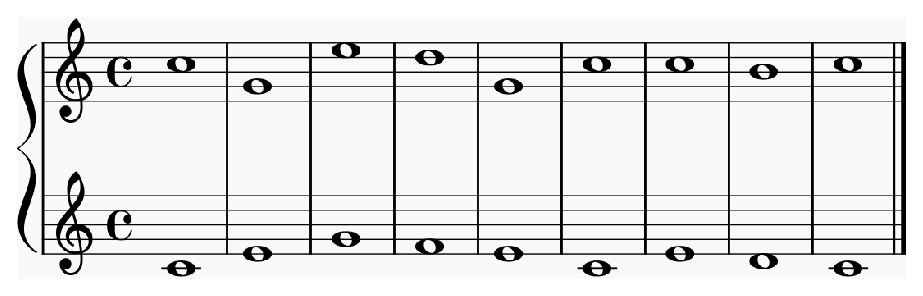
\includegraphics[width=11cm]{figures/first.eps}
\end{frame}

\begin{frame}{Counterpoint: Interaction of Multiple Voices}
\vspace{7mm}
\begin{overpic}[width=11cm]{figures/first.eps}
\put(15,2){\blue{\highbox{\hspace{8cm}}}}
\end{overpic}

\vspace{2mm}

\hspace{4.5cm} cantus firmus
\end{frame}

\begin{frame}{Counterpoint: Interaction of Multiple Voices}
\vspace{-7.3mm}
\hspace{4.5cm} counterpoint

\vspace{2mm}

\begin{overpic}[width=11cm]{figures/first.eps}
\put(15,23){\blue{\highbox{\hspace{8cm}}}}
\end{overpic}
\end{frame}

\begin{frame}{Key Concept 1: Intervals}
\vspace{-7.8mm}
\begin{small}
\hspace{1.5cm} per8\hspace{3mm}min3\hspace{2mm}maj6\hspace{2mm}maj6\hspace{2mm}min3\hspace{2mm}per8\hspace{2mm}maj6\hspace{2mm}maj6\hspace{3mm}per8
\end{small}

\vspace{-3mm}

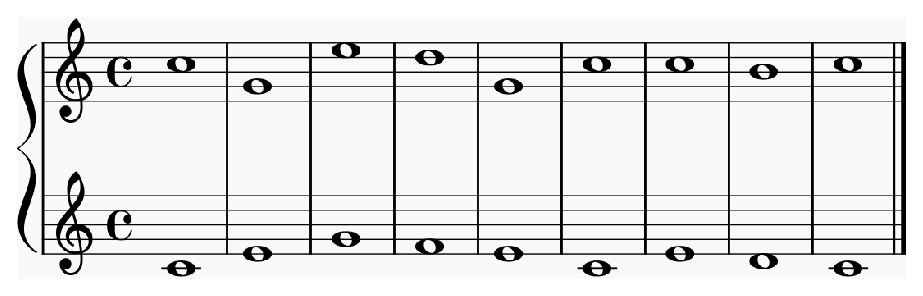
\includegraphics[width=11cm]{figures/first.eps}
\end{frame}

\begin{frame}{Rule 1 for First-Species Counterpoint}
\bscreen{
All intervals must be \empha{consonant}
}

\vspace{-2mm}

\begin{center}
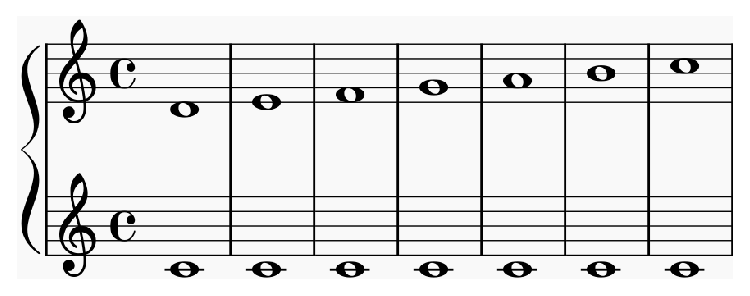
\includegraphics[width=8cm]{figures/interval.eps}
\end{center}

\vspace{-3mm}

\begin{small}
\hspace{2.8cm} 2nd \ \,3rd \ \,4th \ \ 5th \ \,6th \ \ 7th \ \,8th \\
\hspace{2.92cm} $\bad$ \ \ \ \,$\ok$ \ \ \,$\bad$ \ \ \ \ $\ok$ \ \ \ $\ok$ \ \ \ \,$\bad$ \ \ \ $\ok$
\end{small}
\end{frame}

\begin{frame}[fragile]{Representing Valid Intervals}
\begin{small}
\begin{alltt}
\aorange{data} \ablue{IntervalQuality} : \ablue{Set} \aorange{where}
  \agreen{min3}  : \ablue{IntervalQuality}
  \agreen{maj3}  : \ablue{IntervalQuality}
  \agreen{per5}  : \ablue{IntervalQuality}
  \agreen{min6}  : \ablue{IntervalQuality}
  \agreen{maj6}  : \ablue{IntervalQuality}
  \agreen{per8}  : \ablue{IntervalQuality}
  \agreen{min10} : \ablue{IntervalQuality}
  \agreen{maj10} : \ablue{IntervalQuality}

\ablue{PitchInterval} : \ablue{Set}
\ablue{PitchInterval} = \ablue{Pitch \(\times\) IntervalQuality}
\end{alltt}
\end{small}
\end{frame}

\begin{frame}{Key Concept 2: Motion}
\vspace{-1.5mm}
\begin{small}
\hspace{2.2cm} ctr\hspace{6mm}sim\hspace{4mm}par\hspace{5mm}sim\hspace{5mm}ctr\hspace{5mm}obl\hspace{5mm}par\hspace{5.5mm}ctr
\end{small}

\vspace{3mm}

\begin{overpic}[width=11cm]{figures/first.eps}
\end{overpic}

\vspace{3mm}

\begin{small}
\hspace{3mm} where ctr: contrary, sim: similar, par: parallel, obl: oblique
\end{small}
\end{frame}

\begin{frame}{Key Concept 2: Motion}
\vspace{-1.5mm}
\begin{small}
\hspace{2.2cm} \blue{ctr}\hspace{6mm}sim\hspace{4mm}par\hspace{5mm}sim\hspace{5mm}ctr\hspace{5mm}obl\hspace{5mm}par\hspace{5.5mm}ctr
\end{small}

\vspace{3mm}

\begin{overpic}[width=11cm]{figures/first.eps}
\put(20,21){\begin{small}\rotatebox{20}{$\blue{\searrow}$}\end{small}}
\put(20,2){\begin{small}\rotatebox{340}{$\blue{\nearrow}$}\end{small}}
\end{overpic}

\vspace{3mm}

\begin{small}
\hspace{3mm} where ctr: contrary, sim: similar, par: parallel, obl: oblique
\end{small}
\end{frame}

\begin{frame}{Key Concept 2: Motion}
\vspace{-1.5mm}
\begin{small}
\hspace{2.2cm} ctr\hspace{6mm}\blue{sim}\hspace{4mm}par\hspace{5mm}sim\hspace{5mm}ctr\hspace{5mm}obl\hspace{5mm}par\hspace{5.5mm}ctr
\end{small}

\vspace{3mm}

\begin{overpic}[width=11cm]{figures/first.eps}
\put(30,23){\begin{small}\rotatebox{350}{$\blue{\nearrow}$}\end{small}}
\put(29,4){\begin{small}\rotatebox{330}{$\blue{\nearrow}$}\end{small}}
\end{overpic}

\vspace{3mm}

\begin{small}
\hspace{3mm} where ctr: contrary, sim: similar, par: parallel, obl: oblique
\end{small}
\end{frame}

\begin{frame}{Key Concept 2: Motion}
\vspace{-1.5mm}
\begin{small}
\hspace{2.2cm} ctr\hspace{6mm}sim\hspace{4mm}\blue{par}\hspace{5mm}sim\hspace{5mm}ctr\hspace{5mm}obl\hspace{5mm}par\hspace{5.5mm}ctr
\end{small}

\vspace{3mm}

\begin{overpic}[width=11cm]{figures/first.eps}
\put(39,23){\begin{small}\rotatebox{35}{$\blue{\searrow}$}\end{small}}
\put(39,2){\begin{small}\rotatebox{35}{$\blue{\searrow}$}\end{small}}
\end{overpic}

\vspace{3mm}

\begin{small}
\hspace{3mm} where ctr: contrary, sim: similar, par: parallel, obl: oblique
\end{small}
\end{frame}

\begin{frame}{Key Concept 2: Motion}
\vspace{-1.5mm}
\begin{small}
\hspace{2.2cm} ctr\hspace{6mm}sim\hspace{4mm}par\hspace{5mm}sim\hspace{5mm}ctr\hspace{5mm}\blue{obl}\hspace{5mm}par\hspace{5.5mm}ctr
\end{small}

\vspace{3mm}

\begin{overpic}[width=11cm]{figures/first.eps}
\put(68,23){\begin{small}\rotatebox{0}{$\blue{\rightarrow}$}\end{small}}
\put(68,2){\begin{small}\rotatebox{335}{$\blue{\nearrow}$}\end{small}}
\end{overpic}

\vspace{3mm}

\begin{small}
\hspace{3mm} where ctr: contrary, sim: similar, par: parallel, obl: oblique
\end{small}
\end{frame}

\begin{frame}{Rule 2 for First-Species Counterpoint}
\bscreen{
Perfect intervals must be approached \\
by \empha{non-similar motion}
}

\vspace{-2mm}

\begin{center}
\begin{overpic}[width=6cm]{figures/motion.eps}
\put(33,38){\begin{small}\rotatebox{330}{$\blue{\nearrow}$}\end{small}}
\put(34,20){$\bad$}
\put(33,7){\begin{small}\rotatebox{330}{$\blue{\nearrow}$}\end{small}}
\put(73,37){\begin{small}\rotatebox{30}{$\blue{\searrow}$}\end{small}}
\put(73,20){$\bad$}
\put(73,2){\begin{small}\rotatebox{30}{$\blue{\searrow}$}\end{small}}
\end{overpic}
\end{center}

\vspace{-5mm}

\begin{small}
\hspace{4.8cm} per5 \hspace{1.3cm} per8
\end{small}
\end{frame}

\begin{frame}[fragile]{Constraining Motion}
\begin{small}
\begin{alltt}
\ablue{motionOK} : (i1 i2 : \ablue{Interval}) \(\rightarrow\) \ablue{Set}
\ablue{motionOK} i1 i2 \aorange{with} \ablue{motion} i1 i2
         | \ablue{isPerfectInterval} i2
\ablue{motionOK} i1 i2 | \agreen{contrary} | \_     = \ablue{\(\top\)}
\ablue{motionOK} i1 i2 | \agreen{oblique}  | \_     = \ablue{\(\top\)}
\ablue{motionOK} i1 i2 | \agreen{parallel} | \agreen{false} = \ablue{\(\top\)}
\ablue{motionOK} i1 i2 | \agreen{parallel} | \agreen{true}  = \ablue{\(\bot\)}
\ablue{motionOK} i1 i2 | \agreen{similar}  | \agreen{false} = \ablue{\(\top\)}
\ablue{motionOK} i1 i2 | \agreen{similar}  | \agreen{true}  = \ablue{\(\bot\)}
\end{alltt}
\end{small}
\end{frame}

\begin{frame}{Rule 3 for First-Species Counterpoint}
\bscreen{
Final interval must be approached by \\
\empha{contrary step-wise} motion
}

\vspace{-2mm}

\begin{center}
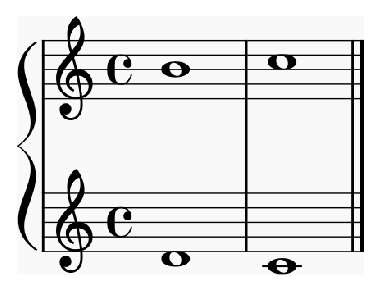
\includegraphics[width=4cm]{figures/cadence2.eps}
\hspace{8mm}
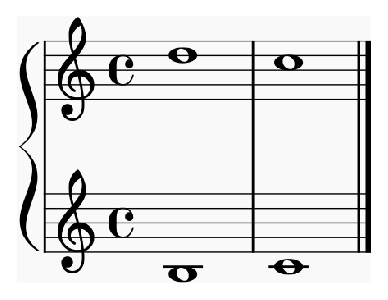
\includegraphics[width=4cm]{figures/cadence7.eps}
\end{center}
\vspace{-4mm}
\begin{small}
\hspace{2.15cm} maj6 \hspace{4cm} min10
\end{small}
\end{frame}

\begin{frame}[fragile]{Building Correct Counterpoint}
\hspace{4.5cm} head element
\begin{small}
\vspace{-3mm}
\begin{alltt}
\aorange{data} \ablue{FirstSpecies} : \ablue{PitchInterval} \(\rightarrow\) \ablue{Set} \aorange{where}
      \(\vdots\)
\end{alltt}
\end{small}
\vspace{4.13cm}
\end{frame}

\begin{frame}[fragile]{Building Correct Counterpoint}
\begin{small}
\begin{alltt}
\aorange{data} \ablue{FirstSpecies} : \ablue{PitchInterval} \(\rightarrow\) \ablue{Set} \aorange{where}
  \agreen{cadence2} : (p : \ablue{Pitch}) \(\rightarrow\)
    \ablue{FirstSpecies} (\ablue{transpose} (\agreen{+} \apurple{2}) p \agreen{,} \agreen{maj6})
  \agreen{cadence7} : (p : \ablue{Pitch}) \(\rightarrow\)
    \ablue{FirstSpecies} (\ablue{transpose} \agreen{-[1+} \apurple{0} \agreen{]} p \agreen{,} \agreen{min10})
      \(\vdots\)
\end{alltt}
\end{small}
\vspace{1.88cm}
\end{frame}

\begin{frame}[fragile]{Building Correct Counterpoint}
\begin{small}
\begin{alltt}
\aorange{data} \ablue{FirstSpecies} : \ablue{PitchInterval} \(\rightarrow\) \ablue{Set} \aorange{where}
  \agreen{cadence2} : (p : \ablue{Pitch}) \(\rightarrow\)
    \ablue{FirstSpecies} (\ablue{transpose} (\agreen{+} \apurple{2}) p \agreen{,} \agreen{maj6})
  \agreen{cadence7} : (p : \ablue{Pitch}) \(\rightarrow\)
    \ablue{FirstSpecies} (\ablue{transpose} \agreen{-[1+} \apurple{0} \agreen{]} p \agreen{,} \agreen{min10})
  \agreen{\_::\_} : (pi : \ablue{PitchInterval}) \(\rightarrow\)
         \{pj : \ablue{PitchInterval}\} \(\rightarrow\)
         \{\_  : \ablue{motionOK} pi pj\} \(\rightarrow\)  \ared{-- implicit}
         \ablue{FirstSpecies} pj \(\rightarrow\)
         \ablue{FirstSpecies} pi
\end{alltt}
\end{small}
\end{frame}

\begin{frame}
\clarge{Demo}
\end{frame}

\begin{frame}{Higher-Species Counterpoint}
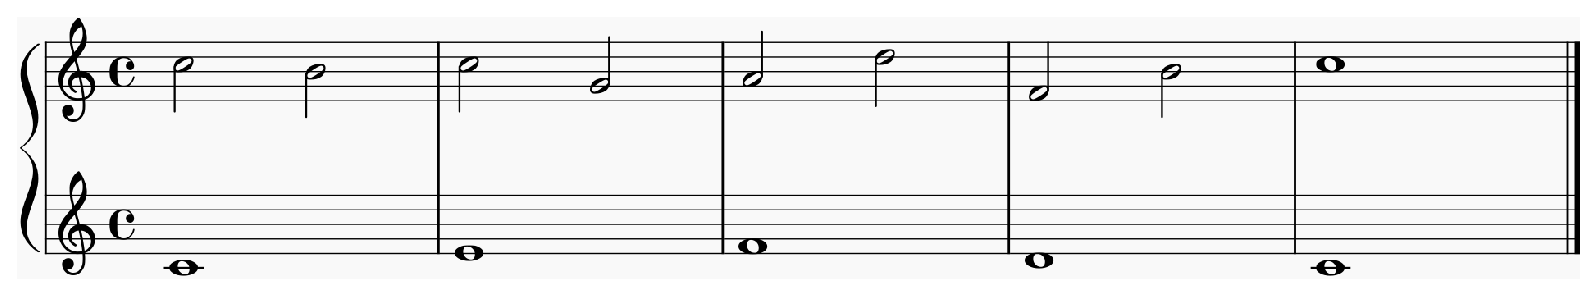
\includegraphics[width=11cm]{figures/second.eps}

\vspace{8mm}

\begin{itemize}
\setlength{\leftskip}{-2mm}
\setlength{\itemsep}{10pt}
\item Counterpoint has more notes than cantus firmus
\item Dissonant intervals are allowed on weak beats
\end{itemize}
\end{frame}

\begin{frame}{Automatic Generation of Counterpoint}
\begin{itemize}
\setlength{\itemsep}{10pt}
\item[\happy] Imperfect intervals
\item[\happy] Varying types of motion
\item[\happy] Contrary motion
\item[\unhappy] Big intervals
\item[\unhappy] Leaps
\item[\unhappy] Repeats
\end{itemize}
\end{frame}

\begin{frame}{Takeaway}
\vspace{-5mm}
\bscreen{
\begin{large}
Compose correct counterpoint \\ 
\vspace{2mm}
using dependent types! 
\end{large}
}

\begin{center}
\url{https://github.com/halfaya/MusicTools}
\end{center}
\end{frame}

% Appendix

\begin{frame}[fragile]{Basic Ingredients}
\begin{alltt}
\aorange{data} \ablue{Pitch} : \ablue{Set} \aorange{where}
  \agreen{pitch} : \(\mathbb{\ablue{N}}\) \(\rightarrow\) \ablue{Pitch}
  
\aorange{data} \ablue{Duration} : \ablue{Set} \aorange{where}
  \agreen{duration} : \(\mathbb{\ablue{N}}\) \(\rightarrow\) \ablue{Duration}
  
\aorange{data} \ablue{Note} : \ablue{Set} \aorange{where}
  \agreen{note} : \ablue{Duration} \(\rightarrow\) \ablue{Pitch} \(\rightarrow\) \ablue{Note}
  \agreen{rest} : \ablue{Duration} \(\rightarrow\)          \ablue{Note}
\end{alltt}
\end{frame}

\begin{frame}[fragile]{Building Music}
\begin{alltt}
\aorange{data} \ablue{Music} : \ablue{Set} \aorange{where}
  \ared{-- single note (base case)}
  \agreen{note} : \ablue{Note}  \(\rightarrow\) \ablue{Music}
  \ared{-- sequential composition}
  \agreen{\_::\_} : \ablue{Music} \(\rightarrow\) \ablue{Music} \(\rightarrow\) \ablue{Music}
  \ared{-- parallel composition}
  \agreen{\_||\_} : \ablue{Music} \(\rightarrow\) \ablue{Music} \(\rightarrow\) \ablue{Music}
\end{alltt}
\end{frame}

\end{document}